%%
%% (
%%  )\ )                             (
%%  (()/(   (            (             )\  )   (
%%   /(_))  ))\   (       ))\  (   (   (()/(   ))\
%%   (_))  /((_)  )\  )  /((_) )\  )\   ((_))/((_)
%%   | _ \(_))(  _(_/( (_) )  ((_)((_)  _| |(_))
%%   |   /| || || ' \))/ -_)/ _|/ _ \/ _` |/ -_)
%%   |_|_\ \_,_||_||_| \___|\__|\___/\__,_|\___|
%%

\documentclass{article}
\usepackage[utf8x]{inputenc}
\usepackage{amsmath}
%\usepackage{slashbox}
\usepackage{amsfonts}
\usepackage{amssymb}
\usepackage{graphicx} % Paquete para incluir imágenes en el documento LaTeX
\usepackage{hyperref}
\hypersetup{
  colorlinks=true,
  linkcolor=blue,
  filecolor=magenta,
  urlcolor=cyan,
}
\urlstyle{same}
\usepackage{varwidth}

\newcommand\tab[1][1cm]{\hspace*{#1}}

\usepackage{multirow}

\usepackage[a4paper,rmargin=1.5cm,lmargin=1.5cm,top=1.5cm,bottom=1.5cm]{geometry}

\usepackage{pdfpages}

\usepackage{xcolor}
\usepackage{minted}
\setminted[cpp]{frame=lines, framesep=2mm, baselinestretch=1.2, rulecolor=\color{black!80}, bgcolor=DarkGray}
\usemintedstyle[cpp]{monokai}
\setminted[python3]{frame=lines, framesep=2mm, baselinestretch=1.2, rulecolor=\color{black!80}, bgcolor=DarkGray}
\usemintedstyle[python]{paraiso-dark}
\setminted[./pseudocode.py:PseudocodeLexer -x]{frame=lines, framesep=2mm, baselinestretch=1.2,
            rulecolor=\color{black!30}, bgcolor=LightGray}
\usemintedstyle[./pseudocode.py:PseudocodeLexer -x]{rainbow_dash}
\setminted[bash]{baselinestretch=1.2,rulecolor=\color{black!30},fontsize=\footnotesize,bgcolor=LightGray}
\definecolor{LightGray}{gray}{0.98}
\definecolor{DarkGray}{gray}{0.1}
\definecolor{MidGray}{gray}{0.8}
\definecolor{codegreen}{rgb}{0,0.6,0}
\definecolor{codegray}{rgb}{0.5,0.5,0.5}
\definecolor{codepurple}{rgb}{0.58,0,0.82}
\definecolor{backcolour}{rgb}{0.95,0.95,0.92}

\setlength{\parindent}{0px}  % Setea la indentacion de la primera linea de cada parrafo a cero pixeles.


\title{Resolución de la novena semana}
\author{@RuneCode}

\begin{document}
%% Portada
\includepdf{./portada/portada.pdf}


%% ####################################################################################
%%    Inicio del Documento
%% ####################################################################################
\section*{Novena Semana}%
En esta clase se revisaron los temas de:
\begin{itemize}
\item \textbf{Arreglo bidimensional}
\item \textbf{Declaración}
\item \textbf{Recorrido}
\item \textbf{Ejemplos}
\end{itemize}
\vspace{1cm}
\textbf{Nota:} Te recomendamos realizar los ejercicios antes de ver su solución
ya que el objetivo de este documento es presentarte una de las muchas posibles
soluciones y así tengas una modelo con el que puedas comparar. Si tienes alguna
sugerencia de mejora puedes comunicarte por correo a la dirección
\href{mailto:gprunecode@gmail.com}{gprunecode@gmail.com}.


\section{Arreglo bidimensional}%
Arreglo de dos dimensiones (Matriz). Está conformado por filas y columnas.

\begin{figure}[h!]
  \centering
  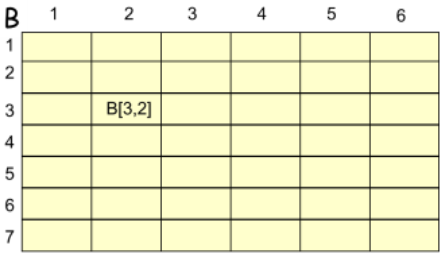
\includegraphics[scale=0.75]{./pictures/arreglo_bidimensional.png}
\end{figure}

\subsection*{Declaración y Referencia (acceso)}%

\subsubsection*{Declaración}%

\begin{minted}{./pseudocode.py:PseudocodeLexer -x}
  Tipo IdenetificadorArreglo [ tamano {, tamano} ]
\end{minted}

\subsubsection*{Referencia a Arreglos}%

\begin{minted}{./pseudocode.py:PseudocodeLexer -x}
  IdentificadorArreglo[ Indice{, Indice} ]
\end{minted}

\subsection*{Recorrido}%
Procesamiento que permite el acceso a todos y cada uno de los elementos del
arreglo bidimensional.\\
Así se puede recorrer todo un arreglo bidimensional para los procesos de:
\begin{itemize}
  \item Leer o asignar valores a todos los elementos del arreglo.
  \item Mostrar o visualizar en pantalla todos los elementos del arreglo.
  \item Sumar todos los elementos del arreglo.
  \item Averiguar por una determinada característica de los elementos del
    arreglo. Como por ejemplo qué números de productos y en qué almacén tienen
    inventario.
\end{itemize}

\subsubsection*{Recorrido por filas}%
Los elementos de la primera fila se procesan primero, a continuación los de la
segunda fila, y así sucesivamente. Sea el arreglo A de 3 filas y 4 columnas.\\

\begin{figure}[h!]
  \centering
  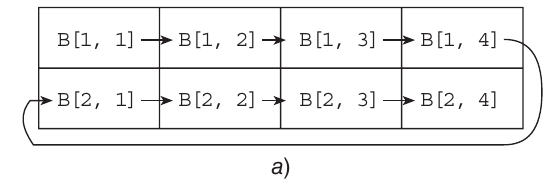
\includegraphics[scale=0.75]{./pictures/recorrido_filas.png}
\end{figure}

Por ejemplo para ingresar datos a una matriz se usaría este procedimiento.

%pseudocodigo
\inputminted{./pseudocode.py:PseudocodeLexer -x}{./pseudocodigo/recorrido_filas.algo}

\subsubsection*{Recorrido por columnas}%
Los elementos de la primera columna se procesan primero, a continuación los de
la segunda columna, y así sucesivamente. Sea el arreglo A de 3 filas y 4
columnas.

\begin{figure}[h!]
  \centering
  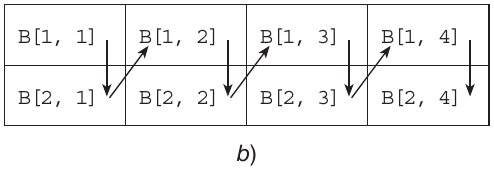
\includegraphics[scale=0.75]{./pictures/recorrido_columna.png}
\end{figure}

Por ejemplo para ingresar datos en una matriz se usará este
procedimiento.\footnotesize{tam representa un número que indica el tamaño
máximo del arreglo.}

%pseudocodigo
\inputminted{./pseudocode.py:PseudocodeLexer -x}{./pseudocodigo/recorrido_columnas.algo}


\subsubsection*{Procedimiento mostrar datos de matriz}%
%pseudocodigo
\inputminted{./pseudocode.py:PseudocodeLexer -x}{./pseudocodigo/mostrar_datos_matriz.algo}

\subsection*{Ejemplo 1}%
Para una matriz de m x n, contar el número de términos positivos, de ceros y de
términos negativos.

%pseudocodigo
\underline{\textit{Resolución en pseudocodigo}}\\
\inputminted{./pseudocode.py:PseudocodeLexer -x}{./pseudocodigo/001_ejemplo.algo}

%C++
\underline{\textit{Resolución en C++}}\\
\inputminted{cpp}{./cpp/Ejemplo.cpp}


\subsubsection*{Ejercicio 1}%
En una matriz de m x n (máximo 50 x 50), almacenar cantidades de tablets vendidas. Se pide:
\begin{itemize}
  \item[a] Hallar el promedio de ventas.
  \item[a] Mostrar cuantas ventas son mayores que el promedio.
\end{itemize}

%pseudocodigo
\underline{\textit{Resolución en pseudocodigo}}\\
\inputminted{./pseudocode.py:PseudocodeLexer -x}{./pseudocodigo/Lab_001.algo}

%pseudocodigo
\underline{\textit{Resolución en pseudocodigo}}\\
\inputminted{./pseudocode.py:PseudocodeLexer -x}{./pseudocodigo/Lab_002.algo}

%pseudocodigo
\underline{\textit{Resolución en pseudocodigo}}\\
\inputminted{./pseudocode.py:PseudocodeLexer -x}{./pseudocodigo/Lab_003.algo}

%pseudocodigo
\underline{\textit{Resolución en pseudocodigo}}\\
\inputminted{./pseudocode.py:PseudocodeLexer -x}{./pseudocodigo/Lab_004.algo}




























\section*{Agradecimientos}
\textbf{Personas que apoyaron mandando psudocódigo y código en este documento:}\\

%---------------------------------------------------------------------------------
\vspace{3cm} 
\section*{¡Envianos tus soluciones!}
Si estás llevando este curso con los profesores Cabrera, Romero o Salinas;
envíanos tus soluciones en los diferentes lenguajes de programación que
conozcas al correo \href{mailto:gprunecode@gmail.com}{gprunecode@gmail.com}.
n.n \\ 

Las mejores soluciones tanto en el algoritmo como en el código, serán
publicadas en las siguientes ediciones de estos documentos.\\

El asunto del correo debe estar de la siguiente manera:\\
$NumeroDeSesion-Profesor-NumeroDeEjercicio$ \\
Por ejemplo:  \\
$01-Romero-01$ \\

Y dentro del correo adjuntar tu solución y nombre como quieras ser reconocido en caso de ser electo.

\vspace{2cm}
\LARGE\textit{RuneCode}


\end{document}

